% Build from the repository root:
% mkdir -p outputs/lewm-evolution-ideas/build
% pdflatex -interaction=nonstopmode -halt-on-error \
%   -output-directory=outputs/lewm-evolution-ideas/build \
%   docs/research/lewm-evolution-ideas.tex
% Copy the built PDF beside this source after visual review.
\documentclass[11pt,a4paper]{article}
\usepackage[margin=21mm,top=19mm,bottom=19mm]{geometry}
\usepackage[T1]{fontenc}
\usepackage{lmodern,microtype,parskip,enumitem,xcolor,tikz,fancyhdr,hyperref}
\usetikzlibrary{arrows.meta}
\definecolor{ink}{HTML}{203443}
\definecolor{accent}{HTML}{246475}
\definecolor{soft}{HTML}{EEF4F5}
\definecolor{muted}{HTML}{53636D}
\hypersetup{colorlinks=true,urlcolor=accent,
  pdftitle={An evolutionary proposal adapter for safe LeWM behaviour},
  pdfauthor={Safety-Dial research notes},
  pdfsubject={A reusable proposal adapter, literature precedents and evaluation questions}}
\pagestyle{fancy}
\fancyhf{}
\fancyhead[L]{\small\color{muted}Safety-Dial\quad /\quad Evolutionary LeWM adapter}
\fancyhead[R]{\small\color{muted}30 October 2026}
\fancyfoot[L]{\small\color{muted}Discussion proposal; not an experiment protocol}
\fancyfoot[R]{\small\color{muted}\thepage\ /\ 2}
\renewcommand{\headrulewidth}{0.3pt}
\renewcommand{\footrulewidth}{0pt}
\setlength{\headheight}{14pt}
\setlength{\parindent}{0pt}
\setlength{\parskip}{7pt}
\setlist[enumerate]{leftmargin=*,itemsep=3pt,topsep=3pt,parsep=0pt}
\setlist[itemize]{leftmargin=*,itemsep=3pt,topsep=3pt,parsep=0pt}
\emergencystretch=1em
\newcommand{\heading}[1]{\par\medskip{\large\bfseries\color{ink}#1}\par\smallskip}
\newcommand{\pagetitle}[2]{{\fontsize{21}{25}\selectfont\bfseries\color{ink}#1\par}
  \vspace{3pt}{\large\color{accent}#2\par}\vspace{5pt}}
\tikzset{stage/.style={draw=accent!45,fill=soft,rounded corners=2pt,
  text width=3.35cm,minimum height=1.05cm,align=center,
  inner sep=5pt,font=\small,text=ink},
  arrow/.style={-{Stealth[length=2mm]},draw=accent,thick}}
\begin{document}
\color{ink}
\pagetitle{An evolutionary adapter for LeWM}{A small controller that learns to propose useful behaviour}

\textbf{Starting point.} LeWM predicts task progress from candidate actions. A
separate learned motion model and supplied geometry predict clearance from newly
introduced hazards. SafeCEM searches for a useful checked plan. The proposal is to
add a small learned controller that supplies better starting action sequences.

\heading{What evolution would learn}
Each individual is a set of adapter-network weights. Given the current observation,
goal and hazard information, the network proposes a short action sequence or a
bounded correction to a proposal. Evolution evaluates candidate networks across
development episodes and improves their weights. The resulting adapter can be
reused in different situations, with its weights fixed during evaluation.

LeWM and the motion predictor remain frozen. SafeCEM refines the proposal using its
existing task score and safety checks. This makes evolution responsible for learning
a behavioural proposal, while preserving the current planning interface.

\begin{center}
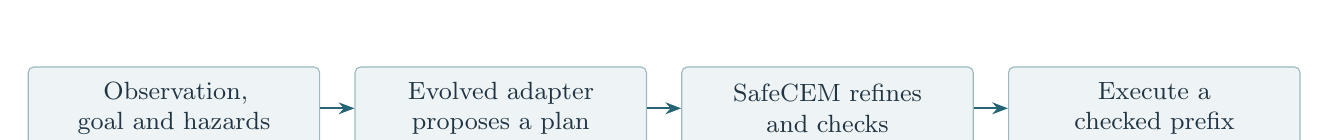
\begin{tikzpicture}
  \node[stage] (a) at (0,0) {Observation,\\goal and hazards};
  \node[stage] (b) at (4.15,0) {Evolved adapter\\proposes a plan};
  \node[stage] (c) at (8.3,0) {SafeCEM refines\\and checks};
  \node[stage] (d) at (12.45,0) {Execute a\\checked prefix};
  \draw[arrow] (a)--(b);
  \draw[arrow] (b)--(c);
  \draw[arrow] (c)--(d);
\end{tikzpicture}
\end{center}

\heading{Training and execution}
\begin{enumerate}
  \item \textbf{Provide causal inputs.} Use world-model features, goal information,
    native proprioception and explicitly supplied hazard geometry. Our virtual hazards
    are not automatically visible in LeWM's images.
  \item \textbf{Evolve network weights.} CMA-ES is one candidate optimizer. Evaluate
    each network with the same frozen models and planner. Rank primarily by actual
    safe task completion, with secondary criteria specified before the experiment.
  \item \textbf{Refine and check each proposal.} SafeCEM also retains ordinary
    proposals so search can recover from a poor adapter. Keep the safety margin and
    prediction allowance fixed. Execute only a checked prefix; refuse if none exists.
  \item \textbf{Freeze before testing.} Select using development evidence, then
    evaluate on fresh source cases without updating adapter weights. Observe and replan
    after each executed prefix.
\end{enumerate}

\heading{Why this might help}
The adapter might learn to propose an initial sideways movement when the direct
route is obstructed. SafeCEM could then refine it into a useful detour. A good
proposal could improve completion or reduce wasted online search. A poor one could
bias search towards an unhelpful route. These are hypotheses; poor initialization
has not been established as the cause of our current stalls.

\textbf{Research question.} Can an evolution-trained proposal adapter improve safe
completion around frozen LeWM under fixed safety requirements and matched budgets?

\textbf{Current status.} This behavioural proposal adapter has not been implemented
or evaluated in our LeWM pipeline. The next page explains the supporting evidence
and the comparisons needed to assess it.

\newpage
\pagetitle{What the literature establishes}{Working precedents and the questions for our study}

\heading{Four close precedents}
\begin{itemize}
  \item \textbf{POPLIN, ICLR 2020 [1].} A policy proposes action sequences for CEM
    refinement; another variant searches policy parameters. Persistent policies use
    cloning, adversarial training or averaging. Models update during training, and
    our hazard-safety setting is not tested.
  \item \textbf{World Models, NeurIPS 2018 [2].} CMA-ES evolves a compact controller
    over learned representations. The CarRacing controller has 867 parameters and
    trains in the actual simulator. A separate VizDoom experiment demonstrates
    learned-model training and transfer. Neither establishes our safe-completion result.
  \item \textbf{Behavior Policy Learning, 2022 [3].} CMA-ES fine-tunes an
    imitation-initialized neural target generator above fixed low-level control.
    One optimized policy completes 8/12 physical pick-and-place configurations.
    This is task completion, not an introduced-hazard safety rate.
  \item \textbf{Safe-LOOP, CoRL 2021 [4].} An actor guides population planning with
    learned dynamics and cost constraints. Actor learning uses gradients and models
    update during training. This supports constrained planning, not evolutionary
    adapter learning specifically.
\end{itemize}

\heading{What to take from these results}
The components have worked, but the complete LeWM combination remains unverified
in this focused search. That is not proof of novelty. Keep existing SafeCEM and learn
a compact proposal. An imitation initialization is worth considering, with its data
and training costs recorded.

POPLIN's parameter-space search can work with fixed zero base weights, so successful
planning alone does not establish useful adapter learning.

\heading{Two separate questions to test}
\begin{enumerate}
  \item \textbf{Does the adapter help?} Compare the same planner alone, with an
    untrained adapter, and with the evolved adapter. If imitation initializes it,
    include the imitation-only adapter before evolutionary fine-tuning.
  \item \textbf{Does evolution add value?} Compare evolution, parameter random
    search and ordinary learning on the same adapter representation, information and
    budgets. Use repeated searches and fresh evaluation source cases.
\end{enumerate}

\textbf{Evidence to retain.} Report safe completion, violations, unfinished episodes
and engagement with denominators. Count training and online work separately and in
total. Predicted feasibility is not guaranteed safety. Training entirely in
imagination needs closed-loop predictions of all inputs and termination, beyond our
current open-loop evaluators.

\vfill
{\footnotesize\color{muted}\setlength{\parskip}{2pt}\textbf{Primary reading}\par
[1] Wang and Ba.
\href{https://arxiv.org/abs/1906.08649}{\emph{Learning to Plan with Policy Networks}}.
ICLR 2020; preprint 2019.\par
[2] Ha and Schmidhuber.
\href{https://worldmodels.github.io/}{\emph{Recurrent World Models Facilitate Policy Evolution}}.
NeurIPS 2018.\par
[3] Tsinganos et al.
\href{https://www.frontiersin.org/journals/robotics-and-ai/articles/10.3389/frobt.2022.974537/full}{\emph{Behavior policy learning}}.
Frontiers in Robotics and AI, 2022.\par
[4] Sikchi, Zhou and Held.
\href{https://proceedings.mlr.press/v164/sikchi22a.html}{\emph{Learning Off-Policy with Online Planning}}.
CoRL 2021; proceedings 2022.}
\end{document}
